\section{Test}
\subsection{Test af Account-klassen}
Der skal laves en test, der sandsynliggør at balancen i Account aldrig kan blive negativ, uanset hvilken værdi set og add metoderne kaldes med. Dvs. en blackbox test af Account-klassen, hvor vi ikke bekymrer os om hvad der sker inde i Account, men blot tester hvad der kommer ud, ift. hvad vi har puttet ind.
\\

Til formålet oprettes en testklasse, ”AccountTesterController”, som tester grænseværdier, store værdier og mere gennemsnitlige værdier. Klassen opretter en ny Account, og kalder derefter ”setAccountValue” og ”addToAccount” med de forskellige værdier. Der udskrives så en kort beskrivelse af hver test, samt resultatet af testen. Herunder outputtet fra metoden.
\begin{figure}[!ht]
\centering
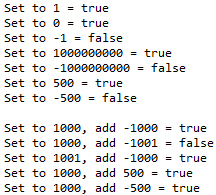
\includegraphics[scale=0.4]{test-illustrationer1.jpg}
\caption[<Text for the list of figures>]{Resultatet af testkørsel}
\label{fig:figure 2} 
\end{figure}
Dvs. hvis kontoen sættes til 1, bliver transaktionen gennemført (metoden returnerer ”true”). Hvis kontoen sættes til 0, bliver transaktionen ligeledes gennemført osv.
\\

Det interessante her er især grænseværdierne, dvs. netop 1, 0 og -1. Testen viser, at klassen opfører sig som vi ville forvente – en positiv værdi giver selvfølgelig true, men mere interessant, 0 giver også true. Ligeledes som forventet, returneres false, hvis balancen sættes til -1.
\\

Når grænseværdierne virker som forventet, vil alle værdier typisk gøre det, men for en sikkerheds skyld testes også lige med nogle meget store værdier, og med nogle helt almindelige værdier. Disse test giver også det forventede resultat.
\\

Herefter udføres en test hvor balancen først sættes til noget kendt, og derefter opdateres med ”addToAccount”. Ved den første test sættes balancen til 1000, hvorefter tilføjes -1000 – således må det forventes at den resulterende balance bliver 0. Dermed vil vi forvente at tranaktionen bliver fuldført, idet 0 ikke er negativt, og dermed er en godkendt værdi. Vi ser, at også denne test giver det forventede resultat.
\\

Sæt til 1000 og tilføj -1001 må give -1, og dermed false – OK.
Sæt til 1001 og tilføj -1000 må give 1, og dermed true – OK.
\\

De mere almindelige værdier giver ligeledes det forventede resultat. Således må det være fair at sige, at det er sandsynligt at en transaktion kun bliver gennemført, hvis ikke den resulterer i en negativ balance.
\\

\subsection{Test og fejlfinding generelt}
Foruden klassen til blackbox-test af Account-klassen, er der udviklet to test-klasser, som kan bruges til fejlfinding og test i programmet. Tanken er, at en eller begge test-klasser kan erstatte de ”rigtige” klasser, og på den måde give en udvikler mulighed for at teste scenarier, som er svære og/eller tidskrævende at opnå ved almindeligt spil.
\\

Der er dels tale om en GameBoard test-klasse, hvor værdierne for felterne alle er negative, således at sikringen af Account-klassen hurtigt kan testes i praksis. Derudover er der tale om en DieCup test-klasse, hvor en udvikler selv har mulighed for at sætte en fast værdi for hvad terningerne skal slå. Således kan der opnås at lande på f.eks. felt nr. 3 (som giver -200) mange gange i træk, og derved teste sikringen af Account-klassen, eller der kan landes på felt 12 (som giver +650) flere gange i træk, og derved teste de handlinger som udføres når en spiller vinder